\documentclass[a4paper]{article}

\usepackage[T1]{fontenc}
\usepackage[utf8]{inputenc}
\usepackage{lmodern}

\usepackage[french]{babel}
\usepackage{graphicx}
\usepackage{xcolor}%				for colors
\usepackage{comment}%				for comment
\usepackage{upquote}%				for quote ''

\usepackage[toc,page]{appendix}

\usepackage{verbatim}%				Insertion de code
\usepackage{framed}%				Pour boite multipage
\usepackage{moreverb}%				Pour extension verbatim

\usepackage{listingsutf8}%				pour le code informatique
\definecolor{mGreen}{rgb}{0,0.6,0}
\definecolor{mGray}{rgb}{0.5,0.5,0.5}
\definecolor{mPurple}{rgb}{0.58,0,0.82}
\definecolor{backgroundColour}{rgb}{0.95,0.95,0.92}

\lstset{
	tabsize=4,
    extendedchars=true,
    breaklines=true,
    keepspaces=true,
	inputencoding=utf8,
    extendedchars=true,
    literate=%
                {é}{{\'e}}{1}%
                {è}{{\`e}}{1}%
                {à}{{\`a}}{1}%
                {ç}{{\c{c}}}{1}%
                {œ}{{\oe}}{1}%
                {ù}{{\`u}}{1}%
                {É}{{\'E}}{1}%
                {È}{{\`E}}{1}%
                {À}{{\`A}}{1}%
                {Ç}{{\c{C}}}{1}%
                {Œ}{{\OE}}{1}%
                {Ê}{{\^E}}{1}%
                {ê}{{\^e}}{1}%
                {î}{{\^i}}{1}%
                {ô}{{\^o}}{1}%
                {û}{{\^u}}{1}%
                {ë}{{\¨{e}}}1
                {û}{{\^{u}}}1
                {â}{{\^{a}}}1
                {Â}{{\^{A}}}1
                {Î}{{\^{I}}}1
}

\lstdefinestyle{PythonStyle}{
    backgroundcolor=\color{backgroundColour},
    commentstyle=\color{mGreen},
    keywordstyle=\color{magenta},
    numberstyle=\tiny\color{mGray},
    stringstyle=\color{mPurple},
    basicstyle=\footnotesize,
    breakatwhitespace=true,
    breaklines=true,
    captionpos=b,
    numbers=left,
    numbersep=5pt,
    language=Python
}

\usepackage{hyperref}%				for HyperText
\hypersetup{
    colorlinks=true,
    linkcolor=black,
    filecolor=magenta,
    urlcolor=cyan,
}
\urlstyle{same}

\title{Projet réseau  TM1A}
\author{AMEEUW Vincent\and CERUTTI Marc}
\date{\today}

%**************************************************************************



\begin{document}


\makeatletter
  \begin{titlepage}
  \centering
      {\large \textsc{Université de Bordeaux}}\\
      \textsc{Licence informatique}\\
    \vspace{1cm}
      
\includegraphics[width=0.5\textwidth]{IMG_Latex/ubx-logo.png}\\
	\vspace{2cm}

\begin{center}
	{\large\textbf{	\@date}}\\
	\vspace{15mm}

    {\Huge   Rapport\\
    \vspace{5mm}
    \textbf{\@title}\\}

    \vspace{15mm}
    {\large AMEEUW Vincent \\ CERUTTI Marc} \\

    \vspace{15mm}
	\begin{abstract}
	\center
	Rapport pour le projet de l'enseignement \\'4TIN401U - Réseaux Info L2' (2017 - 2018) sur la mise en réseau du jeu \textit{Bomberman}\\
	\end{abstract}
\end{center}


  \end{titlepage}
\makeatother


%Table
\cleardoublepage
\tableofcontents

\newpage

%DOC
\part{Préambule}

Dans le cadre de l'enseignement '4TIN401U - Réseaux Info L2' (2017 - 2018) à l'Université de Bordeaux, en semestre 4 de Licence Informatique, nous avons dû adapter le jeu \textit{Bomberman} fait grâce à la bibliothèque Pygame en multijoueur (Description en \ref{moodle}).
\\

Le rendu final de fin d'année fut donc d'avoir un jeu \textit{Bomberman} fonctionnel en langage Python, avec un rapport fait sur notre travail avant \textbf{le vendredi 27 avril à 23h55}.
\\

Le principal objectif de cet enseignement était de nous familiariser sur la mise en réseau de projets informatiques.
Il nous a ainsi permis de mettre en pratique nos connaissances théoriques sur le réseau, la gestion des ports logiciels, des sockets, de l'envoi et de la réception de données ainsi que de leur traitement.
\\

Les contraintes techniques étaient de le faire à l'aide d'un serveur centralisé, qui ne réalise pas d'affichage graphique, mais maintient à jour l'état courant du jeu.
Seuls les clients sont en charge de l'interaction avec l'utilisateur (clavier et affichage graphique) et chaque client dispose d'une copie du modèle, qu'il doit maintenir à jour au travers des échanges réseaux avec le serveur.

	En d'autres termes :
	\begin{itemize}
\item Récupération par le client du modèle serveur à travers le réseau (map, fruits, players).
\item Gestion des connexions / déconnexions des joueurs.
\item Gestion des déplacements des joueurs.
\item Gestion des bombes.
\item Extension à de multiples joueurs.
\item Gestion des erreurs (mort violente d'un client, coupure réseau).
\item Ajout de bonus FUN dans le jeu, impliquant de faire du réseau.
	\end{itemize}


\begin{comment}
Vous devez rendre ici deux fichiers :

    un rapport PDF (de 5 à 10 pages max, police 12) décrivant votre projet, organisé comme cela :
        introduction rapide au projet
        vue d'ensemble fonctionnelle : de ce qui marche parfaitement, de ce qui ne marche pas parfaitement, des bonus et de ce qui reste à faire, ...
        architecture et implémentation : vous prendrez soin de décrire les choix techniques que vous avez effectués (TCP/UDP, select/thread, recv non bloquant, acquittement, ...), ainsi que de décrire votre protocole réseau au moyen d'un formalisme de votre choix (shéma, algorithme en pseudo-langage, automate, ...).
        bilan du projet
    une archive ZIP contenant tous les fichiers sources et ressources (images, ...) utiles au bon fonctionnement de votre projet, ainsi qu'un README détaillant comment lancer et jouer avec votre programme.

La date de rendu est fixée au \textbf{\textcolor{red}{vendredi 27 avril 23h55}}.


\end{comment}

\newpage
\part{Projet réseau}

	\section{Méthode de travail}

	Pour notre méthode de travail, on s'est d'abord mis d'accord sur les protocoles réseau à utiliser et le squelette du code sur papier, puis on a travaillé chacun de notre côté en adaptant le code de l'autre.

	Notre base de code était ainsi assez modulaire pour ne pas avoir de problèmes sur d'éventuelles modifications ou imprévus du code pour la suite.

	\section{Analyse du modèle}

	/**/

	
	\section{Algorithme et implémentation}
		\subsection{Protocoles}
		
\begin{figure}[!htbp]
	\centering
	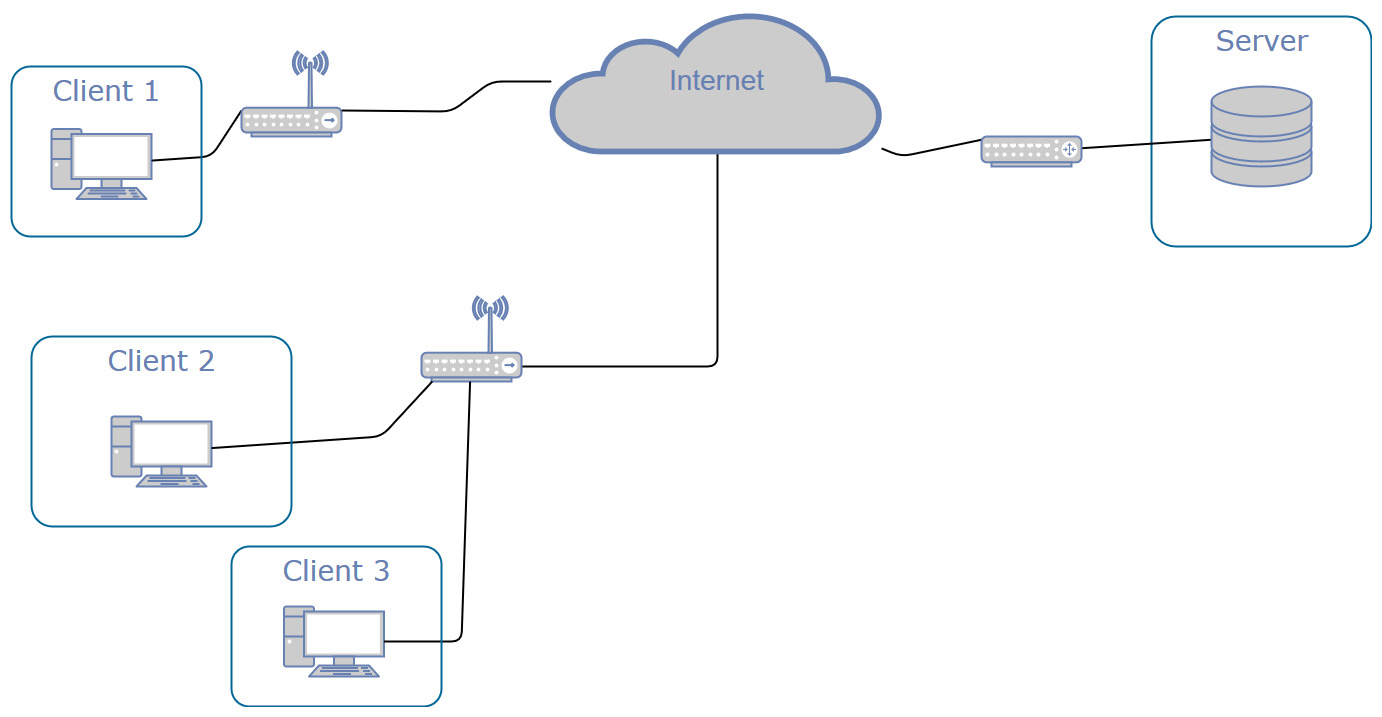
\includegraphics[width=\textwidth]{IMG_Latex/Network.jpg}\\
	\caption{Schéma réseau}
	\label{shema/network}
\end{figure}

\newpage

Tout d'abord nous sommes partis dans l'idée que les clients devait eux mêmes calculé tout ce qui concernait les mouvements, la disparition de fruits et le timer des bombes. Comme on peut supposer que la latence est faible comparé à la vitesse d'interaction des utilisateurs, la différence serait minime.

Cela a cependant eu des répercussions, notamment sur la vie des joueurs où certains ont eu la chance (ou pas) d'être encore en vie sur leur client alors que sur les autres le joueur était mort. Nous avons due donc quand même par sécurité synchroniser les vies des joueurs avec les autres.
\\
\begin{figure}[!htbp]
	\centering
	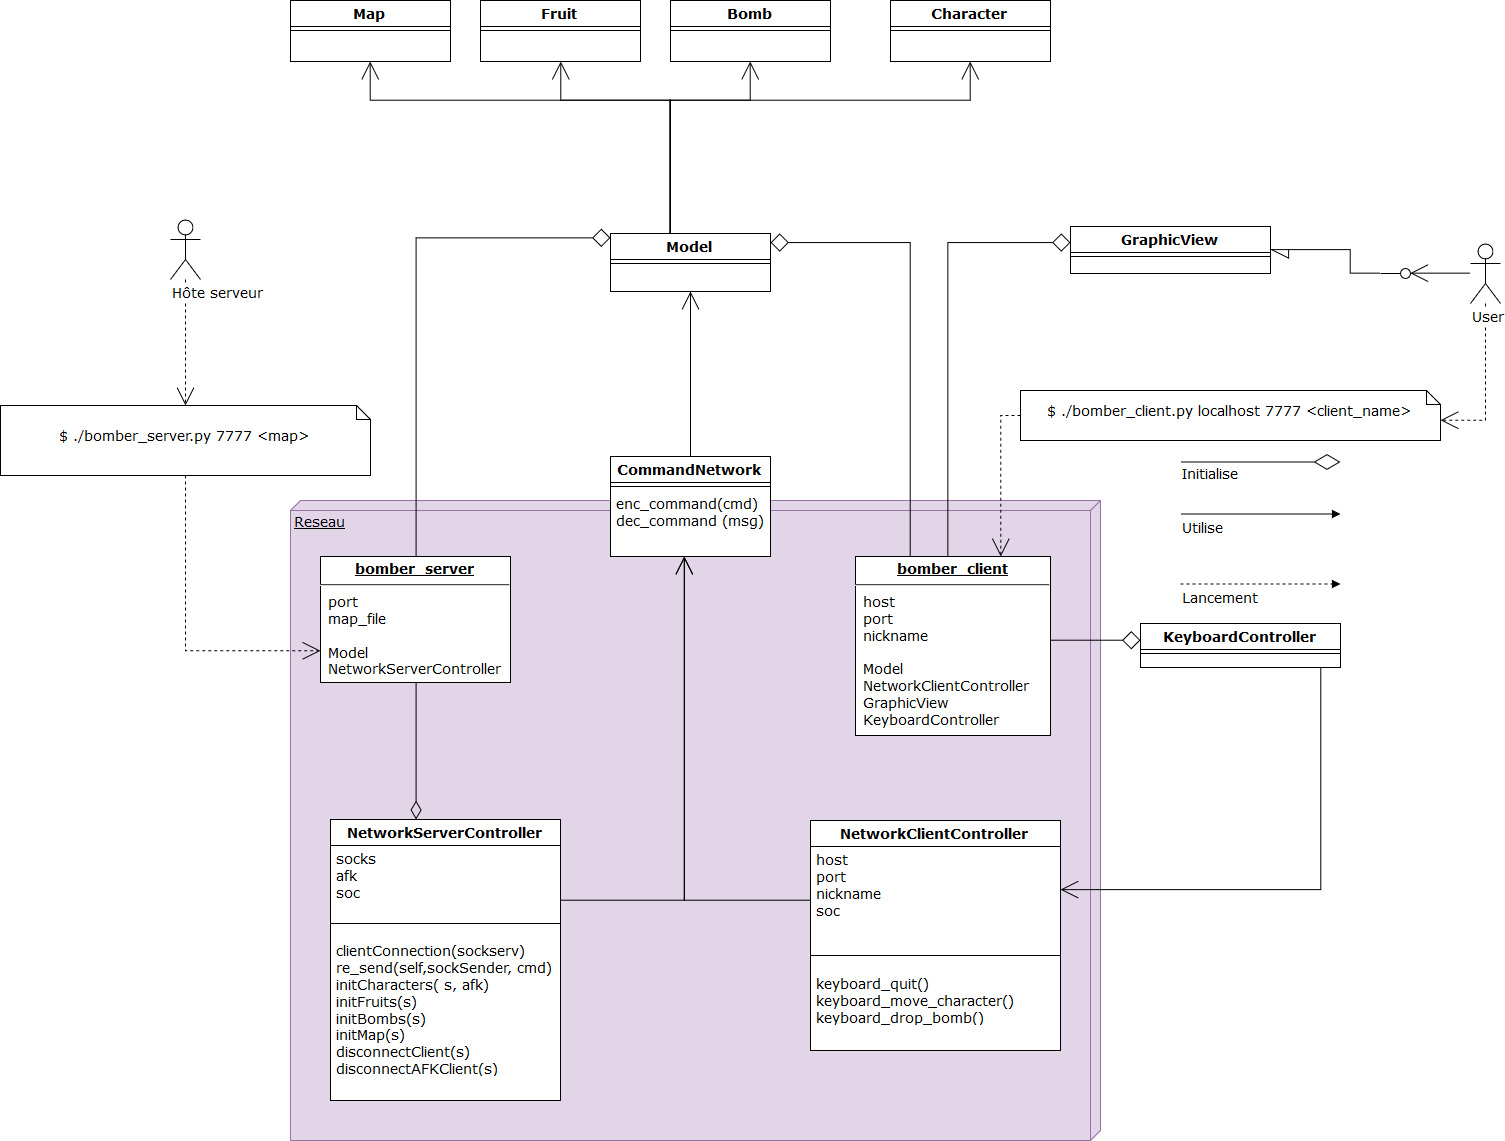
\includegraphics[width=\textwidth]{IMG_Latex/Classes.jpg}\\
	\caption{Schéma simplifié class et dépendances}
	\label{shema/globalproject}
\end{figure}

\newpage
\begin{figure}[!htbp]
	\centering
	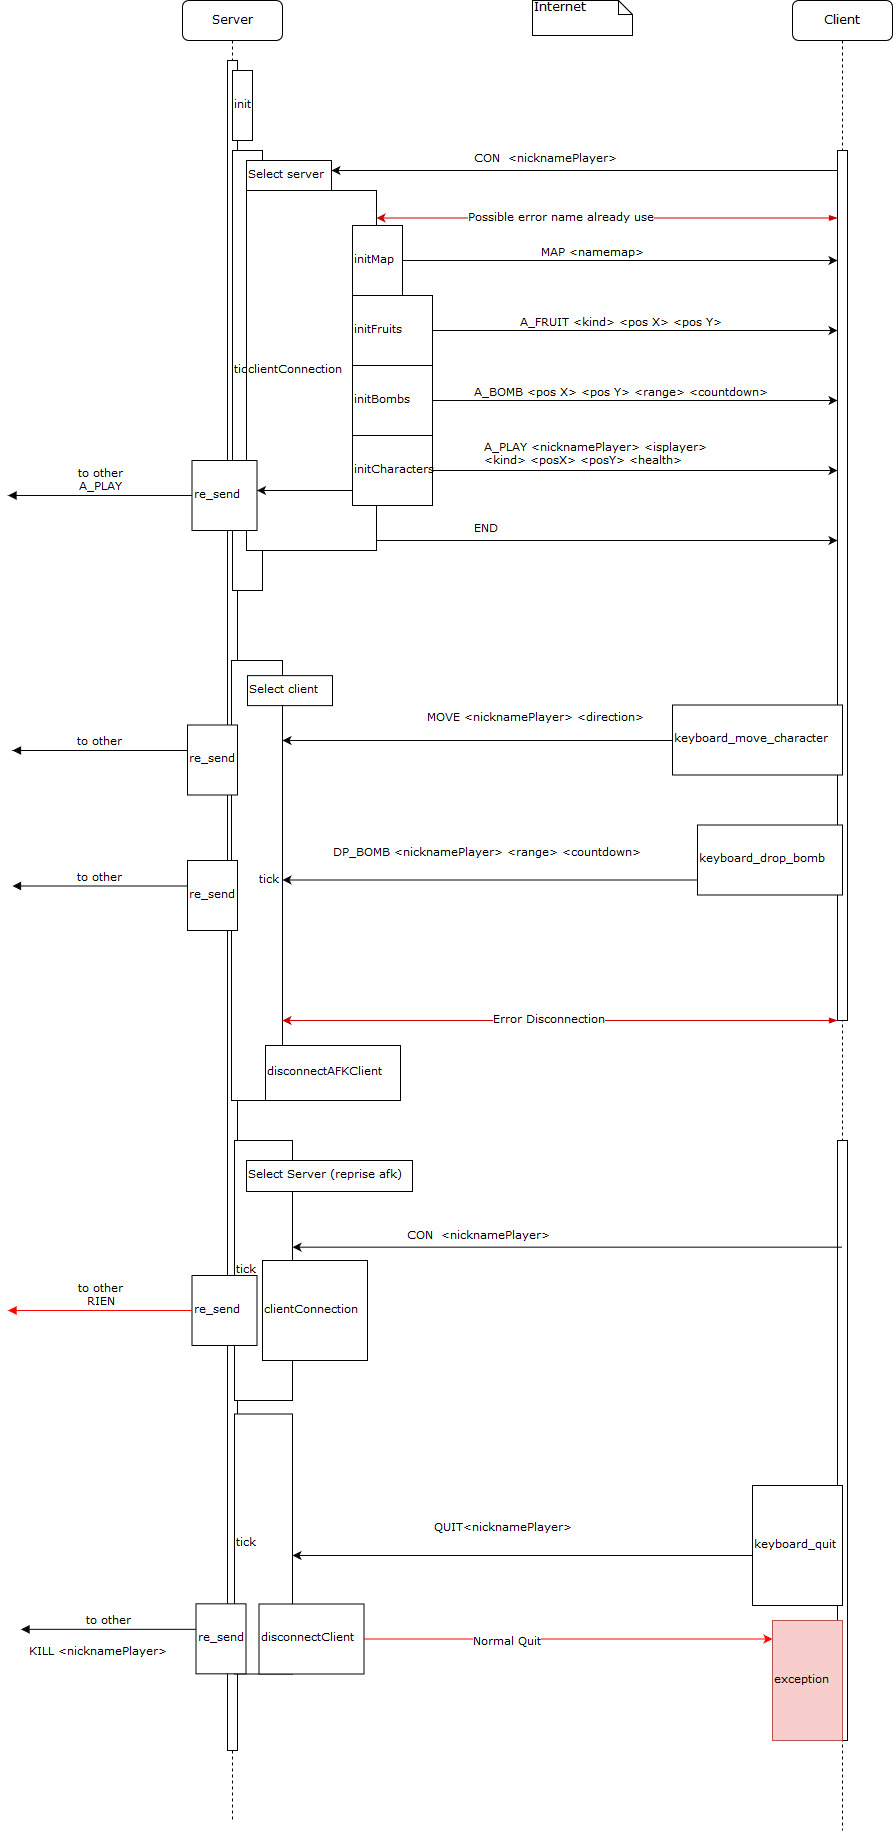
\includegraphics[height=0.9\textheight]{IMG_Latex/ProgrammLifeTime.jpg}\\
	\caption{Schéma simplifié interactions server-client}
	\label{shema/lifeTime}
\end{figure}
		
		
		
\newpage
		\subsection{Choix techniques}
		Nous avons choisi d'utiliser TCP, car ainsi nous évitions de perdre des données en transit nécessaires au bon déroulement du jeu. Cela permettait d'assurer une synchronisation efficace entre les différents copies du jeu.

		En ce qui concerne la gestion des connexions, nous avons choisi d'utiliser select au lieu des threads, car du fait du partage de certaines données comme le model, la liste des sockets, etc, on ne voulait pas "bloquer" ces variables et qu'elles soient disponibles de modifications à n'importe quel moment du jeu sans avoir de problème d'accès. Nous étions plus familier aussi de cet outil grâce au mini-chat réseau\footnote{Travail réalisé durant l'année en réseau.}.

		Puis l'envoi et la réception des données, nous avons choisi d'utiliser les sendall/recv de la bibliotheque socket (\ref{moodle}) en mode non bloquant, car de une, il ne fallait pas bloquer la boucle de jeu pour que tout s'actualise en temps réel, de deux, le sendall permettait de garder un ordre d'envoi chronologique, et nous avons sur les recv gérer quand le buffer recevait plusieurs instructions à la fois.
		
		Ce fut réalisé grâce aux formalismes d'envoi dans la class CommandNetwork, ou on encodait la commande au départ de string en byte array avec enc\_command, et on décodait et on altérait le modèle avec dec\_command, qui vérifier aussi si la commande existait. Les commandes réseau sont de cette forme :
		\textbf{CMD <arg1> <arg2>\textbackslash\textbackslash}
		\\

		Vous avez la liste des commandes en \ref{network.py}

	\section{Améliorations effectuées}
		\subsection{Collisions sur les bombes}
		L'un des principaux problèmes que nous avons rencontré en jouant est que les parties sont longues (il est difficile d'éliminer les autres).
		L'ajout de collisions avec les bombes permet de bloquer les joueurs adverses, les rendant plus simples à éliminer.
		Les parties sont de fait plus courtes mais avec plus d'action.
		\\

		Le principe de cette algorithme est de vérifier pour chaque bombe posé la position d'arrivé du joueur et de celle-ci pour bloquer les mouvements. Nous avions réfléchi à d'autres implémentations en rajoutant sur la map la bombe posé et de vérifier uniquement sur la case d'arrivé du joueur si il y a une bombe, mais cela demanderait beaucoup d'effort pour un petit jeu et plus de mémoire "inutile" si il y a pas de bombes. Comme en plus du fait du timer des bombes et de la période où on peut plus placer de bombes, le nombre de bombes sur le plateau est limité.

		\lstinputlisting[firstline=256,lastline=294, style=PythonStyle]{model.py}

		\subsection{Gestion des déconnexions}
		
		Il y a eu beaucoup de problèmes au niveau de la connection/déconnection des clients. En effet au départ dés que le client fermait (normalement) son jeu, le programme et la socket se fermaient en même temps, ce qui fait que du coté serveur, il ne faisait pas la différence entre une déconnection normal et une brutal.
		
		Nous avons donc en changeant le comportement de l'événement "quit", d'abord envoyer un message au serveur pour se déconnecter, tout en laissant le jeu client tourné jusqu'à que se soit le client qui gère l'erreur du fait de la déconnection par le serveur.
		\\
		L'avantage est que pour la gestion des déconnexions brutales, nous avons choisi que si du coté serveur, un message vide ou une déconnexion impromptue du client se produisait, qu'on fermait la socket associé mais que l'on gardait l'avatar du joueur durant un temps déterminé. Ainsi lors de ce scénario, si l'utilisateur se reconnecte avant le temps déterminé, au lieu de créer un nouveau personnage, il récupère l'ancien.
		
		Le désavantage, c'est que le client si le serveur ferme brutalement ou que il ferme la connection normalement, on peut pas différencier l'erreur.
		

	\section{Bilan et critique}

\newpage
\appendix
\part{Annexes}

\section{Doc python socket} \label{docpysoc}

https://docs.python.org/3/library/socket.html

\section{Moodle} \label{moodle}

https://moodle1.u-bordeaux.fr/course/view.php?id=3671

\section{Github} \label{github}

Professeur
\\
https://github.com/orel33/bomber
\\

Projet
\\
https://github.com/m21-cerutti/VM\_Reseau\_L2
\\

\newpage
\section{Code Source}

\subsection{Network.py} \label{network.py}
\lstinputlisting[style=PythonStyle]{network.py}%firstline=1,lastline=2,
\newpage

\subsection{Model.py} \label{model.py}
\lstinputlisting[style=PythonStyle]{model.py}
\newpage

\subsection{Bomber\textunderscore client.py} \label{bomber_client.py}
\lstinputlisting[style=PythonStyle]{bomber_client.py}
\newpage

\subsection{Bomber\textunderscore server.py} \label{bomber_server.py}
\lstinputlisting[style=PythonStyle]{bomber_server.py}
\newpage

\subsection{Code nécessaire à la compréhension du jeu}
\lstinputlisting[style=PythonStyle]{keyboard.py}
\newpage
\lstinputlisting[style=PythonStyle]{view.py}

\end{document}
